\documentclass[a4paper,11pt]{article}

\usepackage[slovene]{babel}
\usepackage[utf8]{inputenc}

\usepackage{listings}
\usepackage{babelbib}
\usepackage{url}

\usepackage{graphicx}
\usepackage{float}
\graphicspath{ {images/} }
\usepackage[usenames, dvipsnames]{color}

\usepackage{underscore}
\renewcommand{\lstlistingname}{Primer}% Listing -> Primer

\lstset{
numbers=left, 
numberstyle=\small, 
numbersep=8pt, 
frame = single, 
language=Python, 
framexleftmargin=15pt}

\setlength{\parindent}{0pt}
%BORDERS
\usepackage{geometry}
 \geometry{
 a4paper,
 total={170mm,257mm},
 left=30mm,
 right=25mm,
 top=30mm,
 bottom=30mm
 }

\begin{document}
\begin{titlepage}


% ZAČETNA STRAN
\newcommand{\HRule}{\rule{\linewidth}{0.5mm}} % Defines a new command for the horizontal lines, change thickness here

\center % Center everything on the page
 
%----------------------------------------------------------------------------------------
%	HEADING SECTIONS
%----------------------------------------------------------------------------------------

\textsc{ UNIVERZA V MARIBORU\\ FAKULTETA ZA ELEKTROTEHNIKO,\\RAČUNALNIŠTVO IN INFORMATIKO}\\[5cm] % Name of your university/college

%----------------------------------------------------------------------------------------
%	TITLE SECTION
%----------------------------------------------------------------------------------------
{ \huge \bfseries \textbf{POROČILO SPRINTA 1}}\\[0.4cm] % Title of your document
\textsc{\large Povezljivi sistemi in inteligentne storitve}\\[5cm] % Minor heading such as course title

%----------------------------------------------------------------------------------------
%	AUTHORS SECTION
%----------------------------------------------------------------------------------------
{\large Gašper Gračner}\\[0.4cm]
{\large Martin Oprešnik}\\[0.4cm]
{\large Luka Koštomaj}\\[0.4cm] 

%----------------------------------------------------------------------------------------
%	DATE SECTION
%----------------------------------------------------------------------------------------
\vfill % Fill the rest of the page with whitespace
{\large Maribor, Marec 2016}\\[3cm] % Date, change the \today to a set date if you want to be precise
\end{titlepage}
\newpage

%----------------------------------------------------------------------------------------
%	CONTENT SECTION
%----------------------------------------------------------------------------------------

\section{Predvidene naloge}
V prvem sprintu želimo detaljno analizirati podatke in jih pripraviti za nadaljno obdelavo zato planiramo naslednje naloge.
	\begin{enumerate}
		\item{Določitev strukture podatkov - \textcolor{OliveGreen}{DONE},}
		\item{Implematacija parserja - \textcolor{OliveGreen}{DONE},}
		\item{Določitev tipov analiz - \textcolor{OliveGreen}{DONE},}
		\item{Analiza podatkov - \textcolor{OliveGreen}{DONE},}
		\item{Izdelava učne in testne množice}
	\end{enumerate}
\newpage

\section{Implematacija parserja - Martin Oprešnik}


\newpage
\section{Analiza podatkov - Gašper Gračner}
Najprej smo želeli izvedeti količino podatkov glede na športnike, ki jih imamo v našem datasetu, saj nas je zanimo s kakšnimi količinami podatkov za posameznega športnika imamo opravka. \\

\begin{figure}[H]
\caption{Število podatkov glede na športnike}
\centering
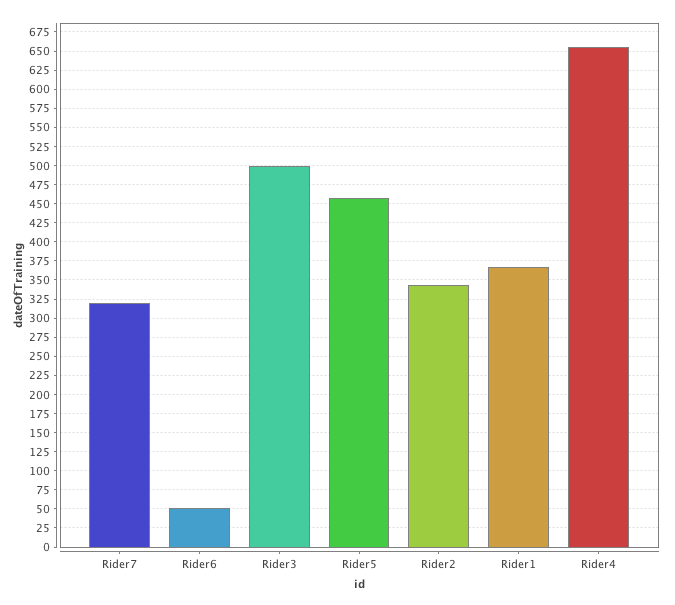
\includegraphics[width=1\textwidth]{ridersTrainingsCount}
\end{figure}

Ker je bila naša naloga razdeliti intenzivnost treninga glede na srčni utrip smo nad podatki povprečnega srčnega utripa zagnali gručenje. S tem postopkom smo dobili tri nivoje intenzivnosti. Za gručenje (K-means) smo se odločili, zaradi pouporabnosti postopka, saj lahko v primeru, da želimo več nivojev le povečamo število K.\\

\begin{figure}[H]
\caption{Gručenje srčnega utripa}
\centering
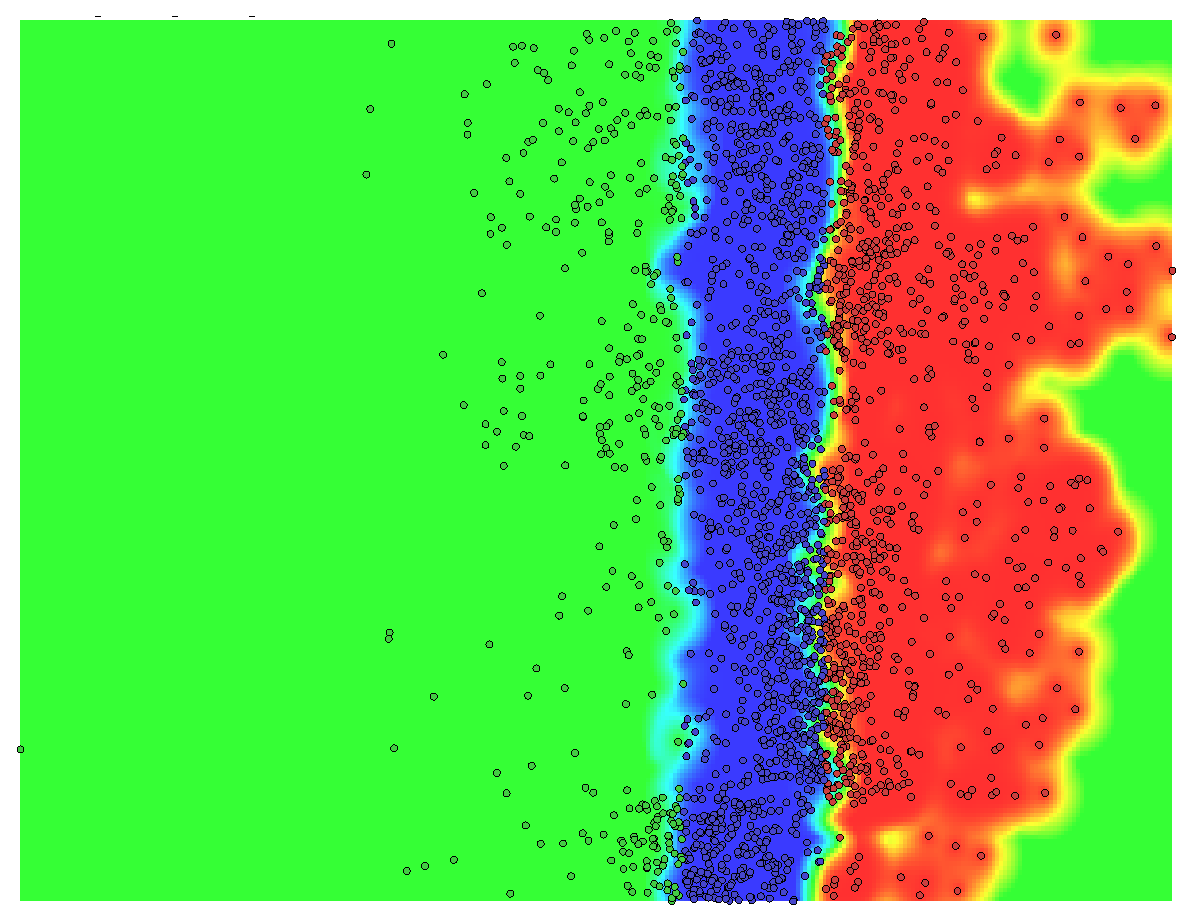
\includegraphics[width=1\textwidth]{HrCLusters}
\end{figure}
 
Rezultat spodaj prikazanega procesa je gručenje in dve .CSV datoteki. Ena z vsemi atributi in druga z samo izbranimi atributi
\begin{enumerate}
\item{Povprečen srčni utrip,}
\item{intenzivnost vadbe,}
\item{id športnika,}
\item{trajanje vadbe}
\item{datum treninga}
\end{enumerate} 

Te podatke smo nato obdelali, tako da smo združili treninge posameznega športnika po tednih. Za vsak dan v tednu smo določili intenzivnost in trajanje treninga. Podatki v tej obliki so pripravljeni za klasifikacijo.

\begin{figure}[H]
\caption{Proces analize podatkov}
\centering
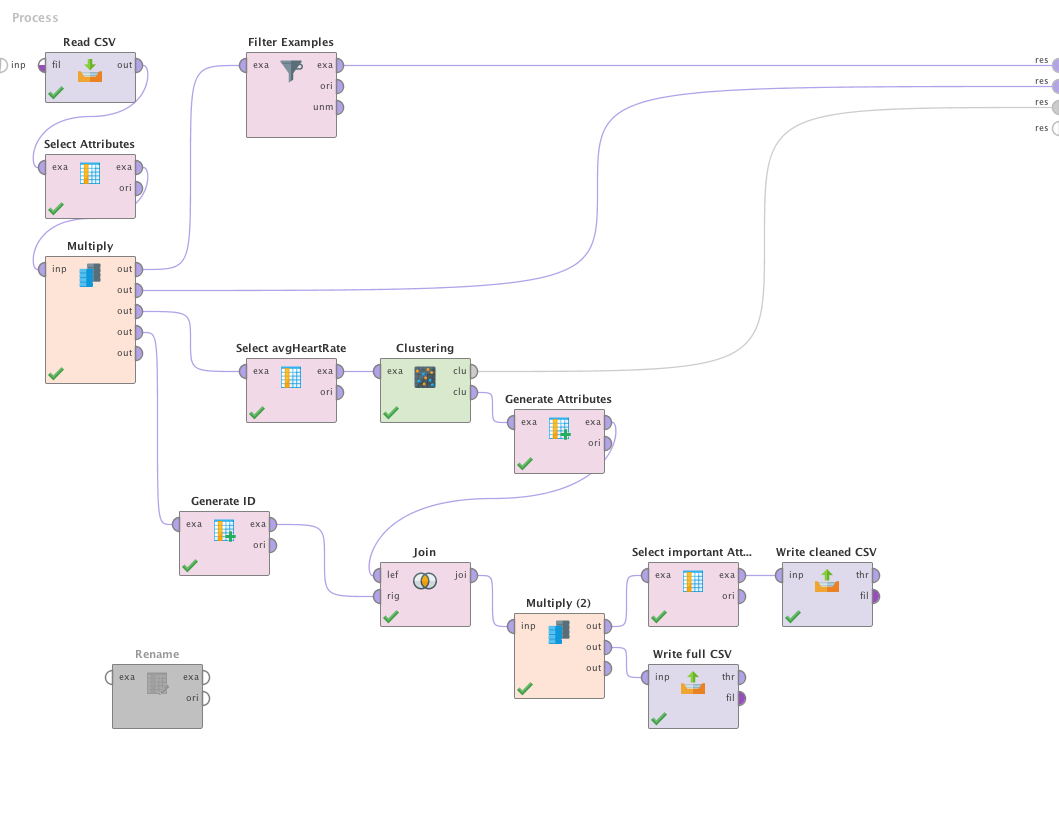
\includegraphics[width=1\textwidth]{IntensityClusteringProcess}
\end{figure}


\newpage
\section{Izdelava učne in testne množice - Luka Koštomaj}




\end{document}